%  PARTIE 2.1 L'ATTENTION

\section{Projet en cours}

\subsection{L'attention}

\paragraph{}L'équipe dont je fais partie étudie particulièrement l'attention. Des hypothèses ont été faites par des chercheurs sur la manière dont elle se manifeste et comment nous
l'utilisons. Le cerveau reçoit en permanence une multitude d'informations de la part de son environnement que l'on appelle des \emph{stimuli}. Il n'est pas capable de traiter tous ces
stimuli dans la durée et doit donc se focaliser sur les informations les plus importantes. A l'heure du numérique, l'être humain a tendance à perdre sa capacité d'attention dans la
durée. En effet, les smartphones et leur notifications par exemple ont tendance à sortir leur propriétaire assez régulièrement de leur tâche en cours. Ce qui entrainerait une chute de
performance sur des taches qui nécessitent une attention prolongée.

\paragraph{}D'après nos observations, nous pensons que l'attention est \emph{sélective}. Elle agit comme un filtre qui se focalise sur ce qui nous parait le plus important parmi les
informations reçues. Elle peut filtrer les informations selon leur aspect spatial, visuel, auditif ... (image de gauche sur la figure \ref{AspectSelectiveAttention}). Par exemple, pour
porter notre focalisation sur un élément visuel, notre attention va faire bouger nos yeux et placer l'élément en plein milieu de notre champs de vision. Cela permet d'avoir des
informations plus détaillées que si l'élément était à la périphérie du champs visuel (image de droite sur la figure \ref{AspectSelectiveAttention}). En même temps, si l'élément est
purement visuel, l'attention va filtrer les informations auditives pour devoir en traiter le moins possible.

\begin{figure}[h]
    \begin{center}
    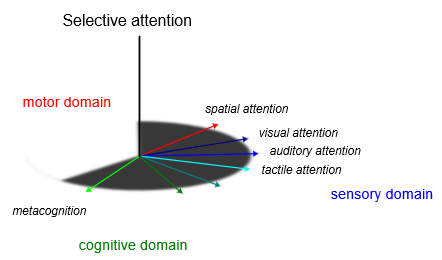
\includegraphics[width=12cm]{selectiveAttention.png}
    \end{center}
    \caption{Les différents aspects de l'attention sélective}
\label{AspectSelectiveAttention}
\end{figure}

\paragraph{}Nous pouvons observer une différences de capacités attentionnelles entre les personnes jeunes et agées. En effet, les jeunes peuvent facilement déplacer leur attention
d'un élément à un autre. C'est \emph{l'attention divisive}. En revanche, ils ont beaucoup de difficultés à la maintenir efficacement dans le temps sur une tâche bien précise. Cette capacité
s'appelle \emph{l'attention soutenue} ou \emph{vigilance}. Les personnes plus agées ont de par leur expèrience une meilleure attention soutenue. Mais, du fait de leur âge, leur attention divise n'est pas
très performante.

\paragraph{}Notre capacité d'attention soutenue dépend de chacun. Plus la tâche est longue et moins il est facile de maintenir son attention. Si la tâche est prévisible, son exécution
va devenir un automatisme et augmentera le risque de vagabondage mental de la personne. Le \emph{vagabondage mental} est un état où la personne a des pensées qui n'ont aucun rapport
avec la tâche qu'elle exécute. Le moment où elle rentre dans l'état de vagabondage est appelé le \emph{décrochage} (voir figure \ref{SustainedAttention}).

\begin{figure}[h]
    \begin{center}
    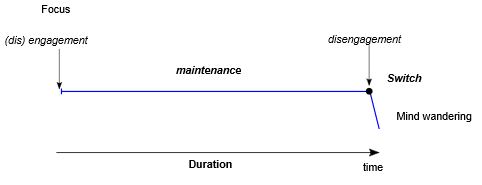
\includegraphics[width=12cm]{sustainedAttention.png}
    \end{center}
    \caption{L'évolution de la vigilance au cours du temps}
\label{SustainedAttention}
\end{figure}

\paragraph{}La difficulté de la tâche rentre aussi en jeu dans le décrochage d'une personne. En effet, si la tâche est trop facile, elle peut devenir prévisible, ennuyeuse et ne
pas nécessiter beaucoup de vigilance. Le sujet va alors rentrer dans un état exécutif plus qu'attentionnel. Mais si celle-ci est trop difficile, elle va demander beaucoup plus de
vigilance et la personne peut décrocher de fatigue, de stress ... Pour de meilleurs performances, il faut également que le rapport effort de vigilance/motivation soit intéressant. Si
ces facteurs de difficulté et de motivation sont bien ajustés, la vigilance peut atteindre un optimum, symbolisant la capactié maximale de la personne (voir figure
\ref{DifficultyAndAttention}) , et qui diffère pour chacun. Cela va nous servir dans le paramétrage des tâches d'entrainement de l'attention dont nous parlerons dans la partie
\ref{TrainingSection}

\begin{figure}[H]
    \begin{center}
    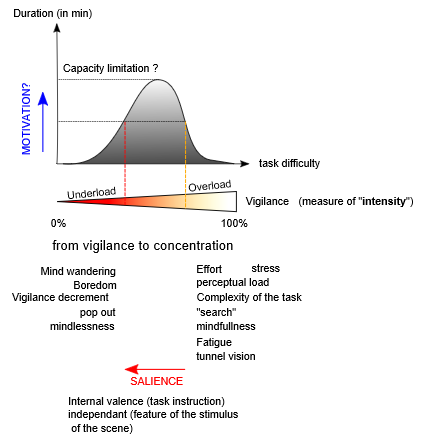
\includegraphics[width=10cm]{difficultyAndAttention.png}
    \end{center}
    \caption{Relation entre la difficulté de la tâche et la vigilance}
\label{DifficultyAndAttention}
\end{figure}

\paragraph{}Il existe une autre facette de l'attention. Celle-ci peut être sollicitée de la même manière tout au long d'une tâche qui ne change pas. Mais il est aussi possible que le
contexte change et que la réalisation de la tâche soit différente. C'est a dire que selon un contexte donné, une action peut être requise ou non. Il faut alors concentrer son
attention sur le fait de s'empécher de faire cette action si le contexte le demande. On appelle cela l'\emph{attention exécutive}. Cet aspect nécessite un certain controle de notre
attention.


\paragraph{}Des études récentes sur des adolescents et des jeunes adultes ont montré un lien entre un usage non modéré des smartphones et surtout des applications de réseaux sociaux
comme Twitter, Facebook ... et une baisse des capacités d'attention soutenue \cite{ART01}. C'est pourquoi notre projet a pour but d'utiliser ces supports censés perturber l'attention
pour l'améliorer grâce à un jeu sérieux d'entrainement.


%  PARTIE 2.2 L'ENTRAINEMENT


\newpage
\subsection{Les taches d'entrainement}
\label{TrainingSection}

\paragraph{}L'amélioration d'une compétence nécessite de l'entrainement. C'est la même chose pour notre attention. Si l'on veut l'améliorer, il faut s'entrainer régulièrement.
L'entrainement de l'attention nécessite la répétition d'une tâche assez difficile pour nécessiter un peu plus que l'attention dont la personne est capable d'utiliser. Elle doit réussir
environ 75\% de la tache (entre 50 et 100\% sans jamais atteindre ces extrêmes) si elle veut s'améliorer.

\paragraph{}Lors de la réalisation d'une tâche, ce sur quoi notre attention doit se porter s'appelle \emph{la cible}. Tous les évênements autres pouvant nous tromper s'appellent
\emph{les distracteurs}. Deux tâches d'expérimentation ont été créées par le doctorant \bsc{Simon Clavagnier} afin de vérifier certains points de l'entrainement.


\subsubsection{La tâche de CPT}

\begin{wrapfigure}[5]{l}{2.3cm}
\vspace{-15pt}
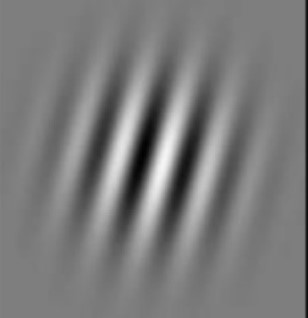
\includegraphics[width=2.3cm]{gabor.jpg}
\end{wrapfigure}

\paragraph{}Le joueur est placé à une distance de 57 cm d'un écran grâce à une mentonnière qui permet de garder une certaine stabilité. Il dispose d'un clavier avec lequel il se sert
uniquement des touches \emph{espace} et \emph{1} et \emph{2} du pavé numérique. Des stimuli sous forme de \glspl{gabor} sont présentés au sujet. La cible est un gabor orienté à
45\degre. Les distracteurs sont des gabors dont l'orientation varie entre 6 et 42\degre par rapport à la cible. Les stimuli apparaissent aléatoirement pendant une période de 80 ms. La
cible a une probabilité d'apparition de 12.5\%. Pour ne pas donner de rythme à l'apparition des stimuli, un temps d'attente de 200ms à 1 seconde les espace.

% - tache principale : dispositif, stimuli : gabor, cible et distracteurs, frequence d'apparition/affichage, action, temps de reaction, son feedback, niveaux : 10 bonnes reponses,
% niveau 7 (dernier niveau) -> discrimation task
% - tache discriminante : vérification sensibilité visuelle, affichage cible/distracteur, choix de reponse, vision centrale et périphérique, assez de données -> tache principale
% N séquences -> 1~2h


\subsubsection{Le gaborium}

La tache de gaborium

%L'équipe dans laquelle je travaille fait des recherches sur l'entrainement de l'attention chez les sujets sains. En effet, on sait qu'il est possible d'entrainer l'attention des
%personnes atteintes de troubles de l'attention mais des recherches sont en cours pour le vérifier chez des sujets sains.

%Le but de l'entrainement existant est d'améliorer l'attention soutenue.

\newpage